\documentclass[
  shownotes,
  xcolor={svgnames},
  hyperref={colorlinks,citecolor=DarkBlue,linkcolor=DarkRed,urlcolor=DarkBlue}
  , aspectratio=169]{beamer}
\usepackage{animate}
\usepackage{amsmath}
\usepackage{amsfonts}
\usepackage{amssymb}
\usepackage{pifont}
\usepackage{mathpazo}
%\usepackage{xcolor}
\usepackage{multimedia}
\usepackage{fancybox}
\usepackage[para]{threeparttable}
\usepackage{multirow}
\setcounter{MaxMatrixCols}{30}
\usepackage{subcaption}
\usepackage{graphicx}
\usepackage{lscape}
\usepackage[compatibility=false,font=small]{caption}
\usepackage{booktabs}
\usepackage{ragged2e}
\usepackage{chronosys}
\usepackage{appendixnumberbeamer}
\usepackage{animate}
\setbeamertemplate{caption}[numbered]
\usepackage{color}
%\usepackage{times}
\usepackage{tikz}
\usepackage{comment} %to comment
%% BibTeX settings
\usepackage{natbib}
\bibliographystyle{apalike}
\bibpunct{(}{)}{,}{a}{,}{,}
\setbeamertemplate{bibliography item}{[\theenumiv]}

% Defines columns for bespoke tables
\usepackage{array}
\newcolumntype{L}[1]{>{\raggedright\let\newline\\\arraybackslash\hspace{0pt}}m{#1}}
\newcolumntype{C}[1]{>{\centering\let\newline\\\arraybackslash\hspace{0pt}}m{#1}}
\newcolumntype{R}[1]{>{\raggedleft\let\newline\\\arraybackslash\hspace{0pt}}m{#1}}


\usepackage{xfrac}


\usepackage{multicol}
\setlength{\columnsep}{0.5cm}

% Theme and colors
\usetheme{Boadilla}

% I use steel blue and a custom color palette. This defines it.
\definecolor{andesred}{HTML}{af2433}

% Other options
\providecommand{\U}[1]{\protect\rule{.1in}{.1in}}
\usefonttheme{serif}
\setbeamertemplate{itemize items}[default]
\setbeamertemplate{enumerate items}[square]
\setbeamertemplate{section in toc}[circle]

\makeatletter

\definecolor{mybackground}{HTML}{82CAFA}
\definecolor{myforeground}{HTML}{0000A0}

\setbeamercolor{normal text}{fg=black,bg=white}
\setbeamercolor{alerted text}{fg=red}
\setbeamercolor{example text}{fg=black}

\setbeamercolor{background canvas}{fg=myforeground, bg=white}
\setbeamercolor{background}{fg=myforeground, bg=mybackground}

\setbeamercolor{palette primary}{fg=black, bg=gray!30!white}
\setbeamercolor{palette secondary}{fg=black, bg=gray!20!white}
\setbeamercolor{palette tertiary}{fg=white, bg=andesred}

\setbeamercolor{frametitle}{fg=andesred}
\setbeamercolor{title}{fg=andesred}
\setbeamercolor{block title}{fg=andesred}
\setbeamercolor{itemize item}{fg=andesred}
\setbeamercolor{itemize subitem}{fg=andesred}
\setbeamercolor{itemize subsubitem}{fg=andesred}
\setbeamercolor{enumerate item}{fg=andesred}
\setbeamercolor{item projected}{bg=gray!30!white,fg=andesred}
\setbeamercolor{enumerate subitem}{fg=andesred}
\setbeamercolor{section number projected}{bg=gray!30!white,fg=andesred}
\setbeamercolor{section in toc}{fg=andesred}
\setbeamercolor{caption name}{fg=andesred}
\setbeamercolor{button}{bg=gray!30!white,fg=andesred}


\usepackage{fancyvrb}
\newcommand{\VerbBar}{|}
\newcommand{\VERB}{\Verb[commandchars=\\\{\}]}
\DefineVerbatimEnvironment{Highlighting}{Verbatim}{commandchars=\\\{\}}
% Add ',fontsize=\small' for more characters per line
\usepackage{framed}
\definecolor{shadecolor}{RGB}{248,248,248}
\newenvironment{Shaded}{\begin{snugshade}}{\end{snugshade}}
\newcommand{\AlertTok}[1]{\textcolor[rgb]{0.94,0.16,0.16}{#1}}
\newcommand{\AnnotationTok}[1]{\textcolor[rgb]{0.56,0.35,0.01}{\textbf{\textit{#1}}}}
\newcommand{\AttributeTok}[1]{\textcolor[rgb]{0.77,0.63,0.00}{#1}}
\newcommand{\BaseNTok}[1]{\textcolor[rgb]{0.00,0.00,0.81}{#1}}
\newcommand{\BuiltInTok}[1]{#1}
\newcommand{\CharTok}[1]{\textcolor[rgb]{0.31,0.60,0.02}{#1}}
\newcommand{\CommentTok}[1]{\textcolor[rgb]{0.56,0.35,0.01}{\textit{#1}}}
\newcommand{\CommentVarTok}[1]{\textcolor[rgb]{0.56,0.35,0.01}{\textbf{\textit{#1}}}}
\newcommand{\ConstantTok}[1]{\textcolor[rgb]{0.00,0.00,0.00}{#1}}
\newcommand{\ControlFlowTok}[1]{\textcolor[rgb]{0.13,0.29,0.53}{\textbf{#1}}}
\newcommand{\DataTypeTok}[1]{\textcolor[rgb]{0.13,0.29,0.53}{#1}}
\newcommand{\DecValTok}[1]{\textcolor[rgb]{0.00,0.00,0.81}{#1}}
\newcommand{\DocumentationTok}[1]{\textcolor[rgb]{0.56,0.35,0.01}{\textbf{\textit{#1}}}}
\newcommand{\ErrorTok}[1]{\textcolor[rgb]{0.64,0.00,0.00}{\textbf{#1}}}
\newcommand{\ExtensionTok}[1]{#1}
\newcommand{\FloatTok}[1]{\textcolor[rgb]{0.00,0.00,0.81}{#1}}
\newcommand{\FunctionTok}[1]{\textcolor[rgb]{0.00,0.00,0.00}{#1}}
\newcommand{\ImportTok}[1]{#1}
\newcommand{\InformationTok}[1]{\textcolor[rgb]{0.56,0.35,0.01}{\textbf{\textit{#1}}}}
\newcommand{\KeywordTok}[1]{\textcolor[rgb]{0.13,0.29,0.53}{\textbf{#1}}}
\newcommand{\NormalTok}[1]{#1}
\newcommand{\OperatorTok}[1]{\textcolor[rgb]{0.81,0.36,0.00}{\textbf{#1}}}
\newcommand{\OtherTok}[1]{\textcolor[rgb]{0.56,0.35,0.01}{#1}}
\newcommand{\PreprocessorTok}[1]{\textcolor[rgb]{0.56,0.35,0.01}{\textit{#1}}}
\newcommand{\RegionMarkerTok}[1]{#1}
\newcommand{\SpecialCharTok}[1]{\textcolor[rgb]{0.00,0.00,0.00}{#1}}
\newcommand{\SpecialStringTok}[1]{\textcolor[rgb]{0.31,0.60,0.02}{#1}}
\newcommand{\StringTok}[1]{\textcolor[rgb]{0.31,0.60,0.02}{#1}}
\newcommand{\VariableTok}[1]{\textcolor[rgb]{0.00,0.00,0.00}{#1}}
\newcommand{\VerbatimStringTok}[1]{\textcolor[rgb]{0.31,0.60,0.02}{#1}}
\newcommand{\WarningTok}[1]{\textcolor[rgb]{0.56,0.35,0.01}{\textbf{\textit{#1}}}}
\usepackage{graphicx}
\makeatletter

\definecolor{airforceblue}{rgb}{0.36, 0.54, 0.66}

\usepackage{tikz}
% Tikz settings optimized for causal graphs.
\usetikzlibrary{shapes,decorations,arrows,calc,arrows.meta,fit,positioning}
\tikzset{
    -Latex,auto,node distance =1 cm and 1 cm,semithick,
    state/.style ={ellipse, draw, minimum width = 0.7 cm},
    point/.style = {circle, draw, inner sep=0.04cm,fill,node contents={}},
    bidirected/.style={Latex-Latex,dashed},
    el/.style = {inner sep=2pt, align=left, sloped}
}


\makeatother






%%%%%%%%%%%%%%% BEGINS DOCUMENT %%%%%%%%%%%%%%%%%%

\begin{document}

\title[Lecture 5]{Lecture 5: \\ Aprendizaje No Supervizado}
\subtitle{Aprendizaje y Minería de Datos para los Negocios}
\date{\today}

\author[Sarmiento-Barbieri]{Ignacio Sarmiento-Barbieri}
\institute[Uniandes]{Universidad de los Andes}


\begin{frame}[noframenumbering]
\maketitle
\end{frame}

%%%%%%%%%%%%%%%%%%%%%%%%%%%%%%%%%%%



%----------------------------------------------------------------------% 

\begin{frame}
\frametitle{Agenda}

\tableofcontents

\end{frame}

%----------------------------------------------------------------------%
\section{Tipos de Aprendizaje}
%----------------------------------------------------------------------%
 \begin{frame}[noframenumbering]
\tableofcontents[currentsubsection]

\end{frame}
%----------------------------------------------------------------------%
\begin{frame}
\frametitle{Tipos de Aprendizaje}
\begin{itemize}


\item ML se divide en dos (¿?) ramas principales:
\medskip
  \begin{enumerate}

  \item Aprendizaje supervisado: Tenemos datos tanto sobre un resultado $y$ como sobre las variables explicativas $X$.
    \begin{itemize}
      \item Esto es lo más cercano al análisis de regresión que conocemos. 
      \item Si $y$ es discreto, también podemos ver esto como un problema de clasificación.
      
    \end{itemize}


  \pause
  \item  Aprendizaje no supervisado: No tenemos datos sobre $y$, solo sobre $X$.
  \item Lo utilizamos generalmente para 2 tareas:
  \begin{itemize}
    \item Permite reducir la dimensionalidad y explorar datos
    \item Agrupar datos
  \end{itemize}

  \end{enumerate}
\end{itemize}
\end{frame}

%----------------------------------------------------------------------%
\section{Reducción de Dimensión: PCA}
%----------------------------------------------------------------------%
\begin{frame}
\frametitle{Exploración de Caracteristicas}
\framesubtitle{Ejemplo: Casas}


\begin{itemize}
  \item Comencemos con un ejemplo simple
  \item Tenemos un grupo de 100 casas y características de estas casas
  \item Queremos hacer un análisis exploratorio y no sabemos donde comenzar
  \item Tenemos las siguientes variables
\end{itemize}
\begin{figure}[H] \centering

    \centering
    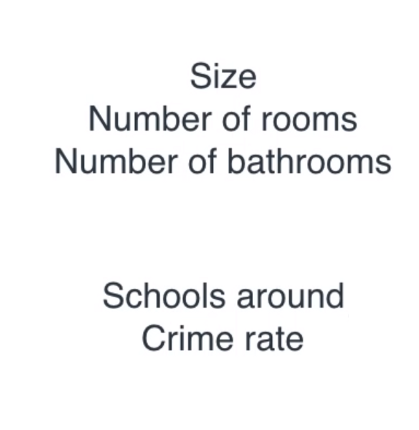
\includegraphics[scale=.35]{figures/pca0}
  \\
  \tiny
\end{figure}

\end{frame}

%----------------------------------------------------------------------%
\begin{frame}
\frametitle{Exploración de Caracteristicas}



% A modo de ejemplo, supongamos que disponemos de una base de datos de 100
% clientes de un banco que cuenta con información sobre 10 variables que
% miden riesgo crediticio de los clientes. Estas variables contienen
% información sobre transacciones bancarias, historia crediticia, entre
% otras. La pregunta que queremos responder es si es posible construir una
% suerte de índice que permita condensar todas estas dimensiones en una
% sola que resuma el riesgo crediticio.

% La primer respuesta obvia sería construir un índice compuesto por el
% promedio de estas 10 variables. Sin embargo, todas estas variables
% pueden contener información redundante o no tener la misma importancia.
% El problema entonces se puede pensar como cuál es la mejor forma de
% construir este índice combinando linealmente estas variables.



\begin{itemize}
\item Supongamos que queremos visualizar \(n\) observaciones de las cuales tenemos \(k\) variables o atributos, representadas por \(x_1,x_2,\dots,x_k\) como parte de un análisis descriptivo. 


\begin{figure}[H] \centering

    \centering
    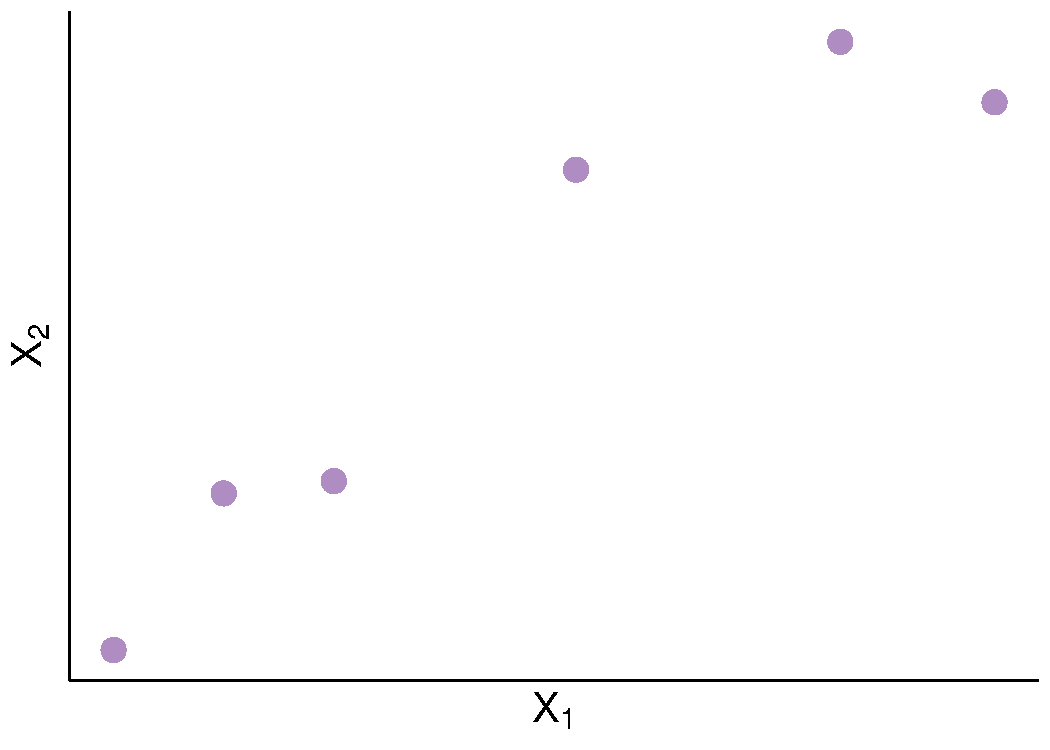
\includegraphics[scale=.35]{figures/plot1ba}
  \\
  \tiny
\end{figure}
\end{itemize}



\end{frame}

%----------------------------------------------------------------------%
\begin{frame}
\frametitle{Exploración de Caracteristicas}



% A modo de ejemplo, supongamos que disponemos de una base de datos de 100
% clientes de un banco que cuenta con información sobre 10 variables que
% miden riesgo crediticio de los clientes. Estas variables contienen
% información sobre transacciones bancarias, historia crediticia, entre
% otras. La pregunta que queremos responder es si es posible construir una
% suerte de índice que permita condensar todas estas dimensiones en una
% sola que resuma el riesgo crediticio.

% La primer respuesta obvia sería construir un índice compuesto por el
% promedio de estas 10 variables. Sin embargo, todas estas variables
% pueden contener información redundante o no tener la misma importancia.
% El problema entonces se puede pensar como cuál es la mejor forma de
% construir este índice combinando linealmente estas variables.



\begin{itemize}

\item Siguiendo el ejemplo anterior, \(n\) serian las 100 casas  y \(k\) las 5 variables que miden caracteristicas de las casas. 
\medskip
\item Una forma de hacer el análisis descriptivo es haciendo diagramas de dispersión para las \(n\) observaciones examinando dos variables por vez.
\medskip
\item  El problema surge que vamos a tener

\begin{align}
\left(\left(\begin{array}{c} 5\\ 2 \end{array}\right)=\frac{5\times4}{2}=10\right)
\end{align}

\item Si fuesen 10 tendriamos 45, y 20, 190!

\end{itemize}
% Si \(k\) es muy grande, como suele serlo en estas aplicaciones, sería imposible examinar todas las graficas. Necesitamos un método que nos permita visualizar cuando la dimensión \(k\) es muy grande. El análisis de componentes principales es una herramienta que nos permite alcanzar
% este objetivo.

% Intuitivamente, PCA plantea que cada observación se encuentra en un
% espacio \(k-dimensional\), pero en el que no todas estas dimensiones son
% igualmente informativas. Por lo tanto, PCA busca representar los datos
% en un espacio de menor dimensión, reteniendo la mayor cantidad de
% información posible. Entonces estas nuevas dimensiones encontradas por
% PCA, llamadas componentes, es una combinación lineal de las variables
% originales.
\end{frame}
%----------------------------------------------------------------------%
\begin{frame}
\frametitle{Reduccion de Dimension: PCA}


\begin{itemize}
  \item PCA: análisis de componentes principales
\medskip
\item Es una técnica de aprendizaje no supervisado que permite reducir la dimensionalidad de tales conjuntos de datos, aumentando la
interpretabilidad, pero al mismo tiempo minimizando la pérdida de información. 
\medskip
\item Intuitivamente, PCA plantea que cada observación se encuentra en un  espacio \(k-dimensional\), pero en el que no todas estas dimensiones son igualmente informativas. 

\end{itemize}
\end{frame}
%----------------------------------------------------------------------%
\begin{frame}
\frametitle{Reduccion de Dimension: PCA}

\begin{itemize}
\item Por lo tanto, PCA busca representar los datos en un espacio de menor dimensión, reteniendo la mayor cantidad de  información posible.
\medskip

\item  Entonces estas nuevas dimensiones encontradas por PCA, llamadas componentes, es una combinación lineal de las variables  originales.
\medskip
\item Se han desarrollado muchas técnicas para este propósito, pero el análisis de componentes principales es uno de los más antiguos y más utilizados. 


\end{itemize}


\end{frame}
%----------------------------------------------------------------------%
\begin{frame}
\frametitle{Reduccion de Dimension: PCA}

\begin{figure}[H] \centering

    \centering
    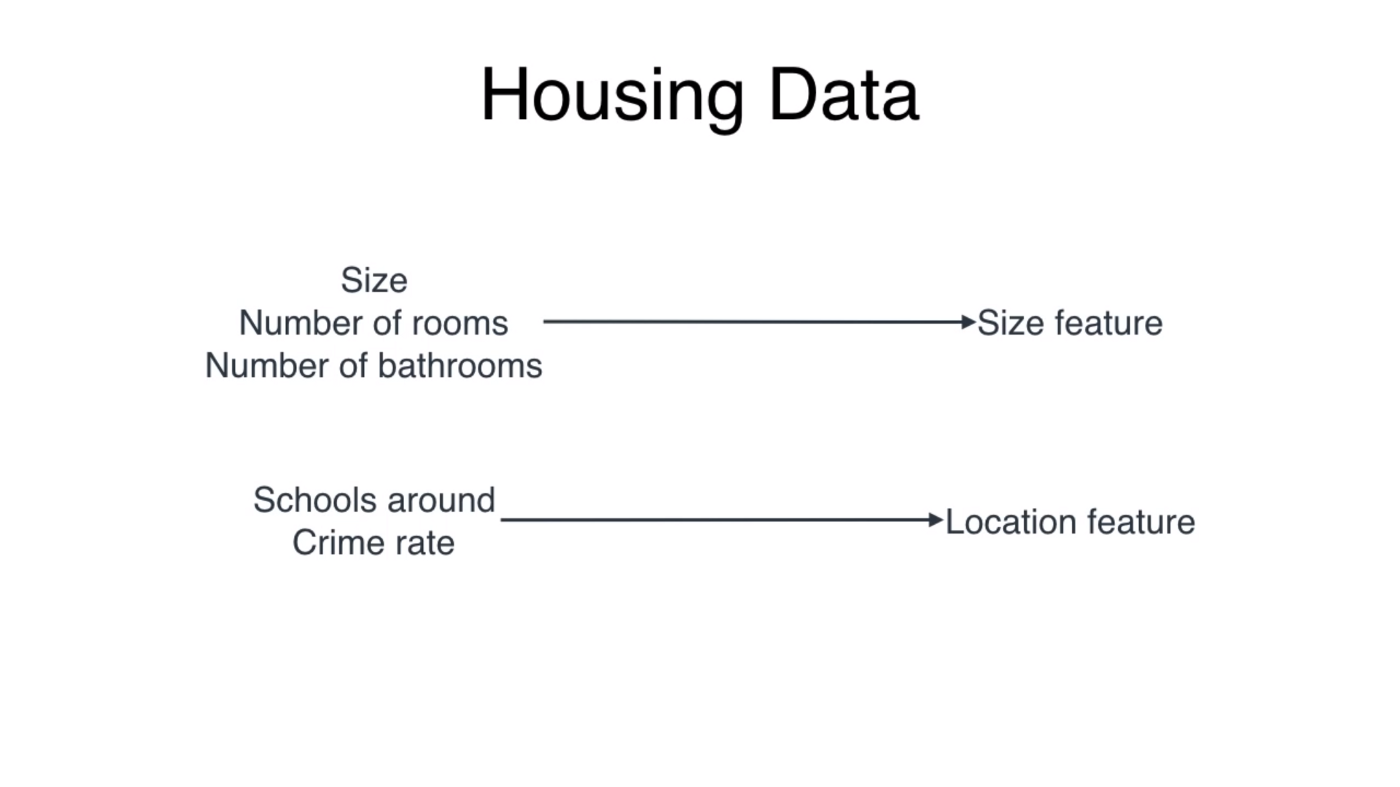
\includegraphics[scale=.25]{figures/pca1}
  \\
  \tiny
\end{figure}


\end{frame}
%----------------------------------------------------------------------%
\begin{frame}
\frametitle{Reduccion de Dimension: PCA}

\begin{figure}[H] \centering

    \centering
    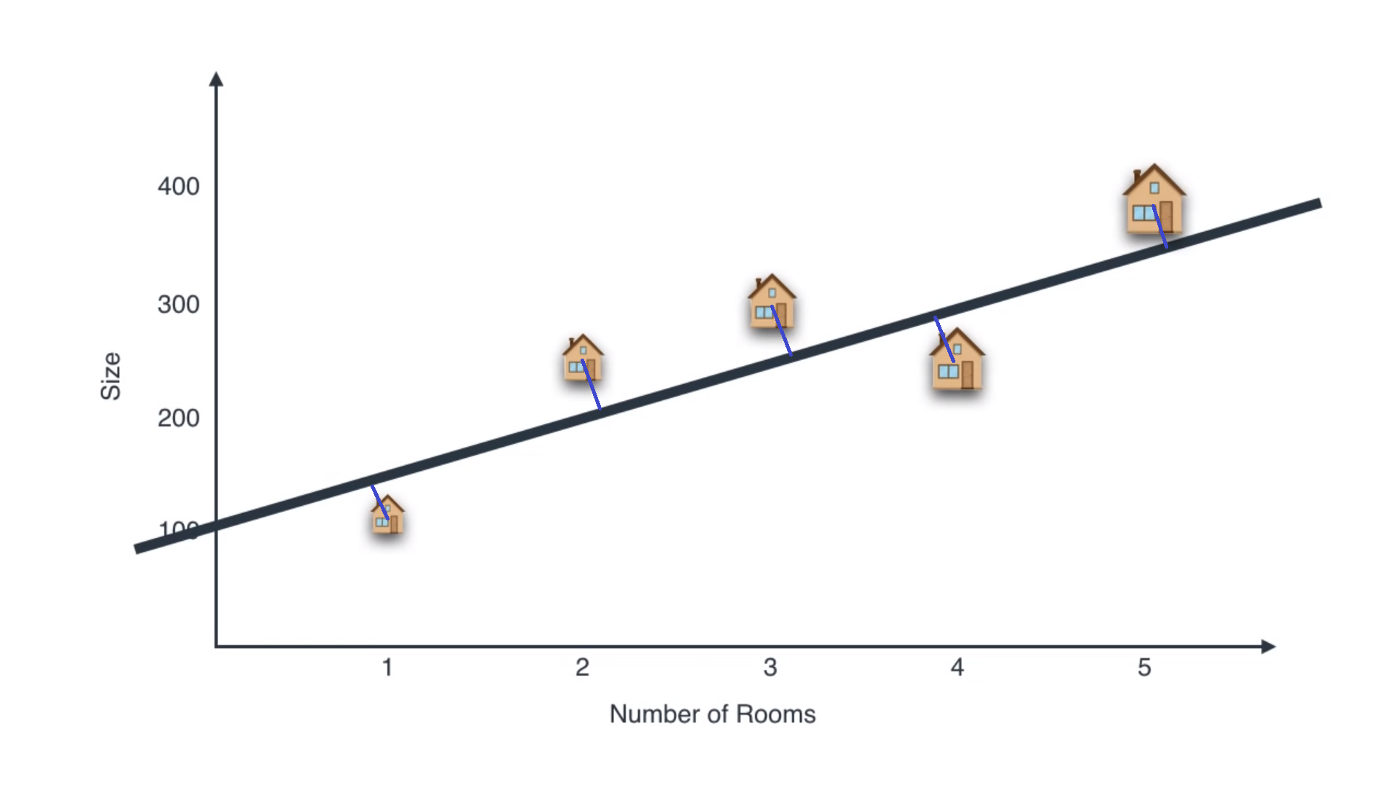
\includegraphics[scale=.25]{figures/pca2}
  \\
  \tiny
\end{figure}



\end{frame}
%----------------------------------------------------------------------%
\begin{frame}
\frametitle{Reduccion de Dimension: PCA}

\begin{figure}[H] \centering

    \centering
    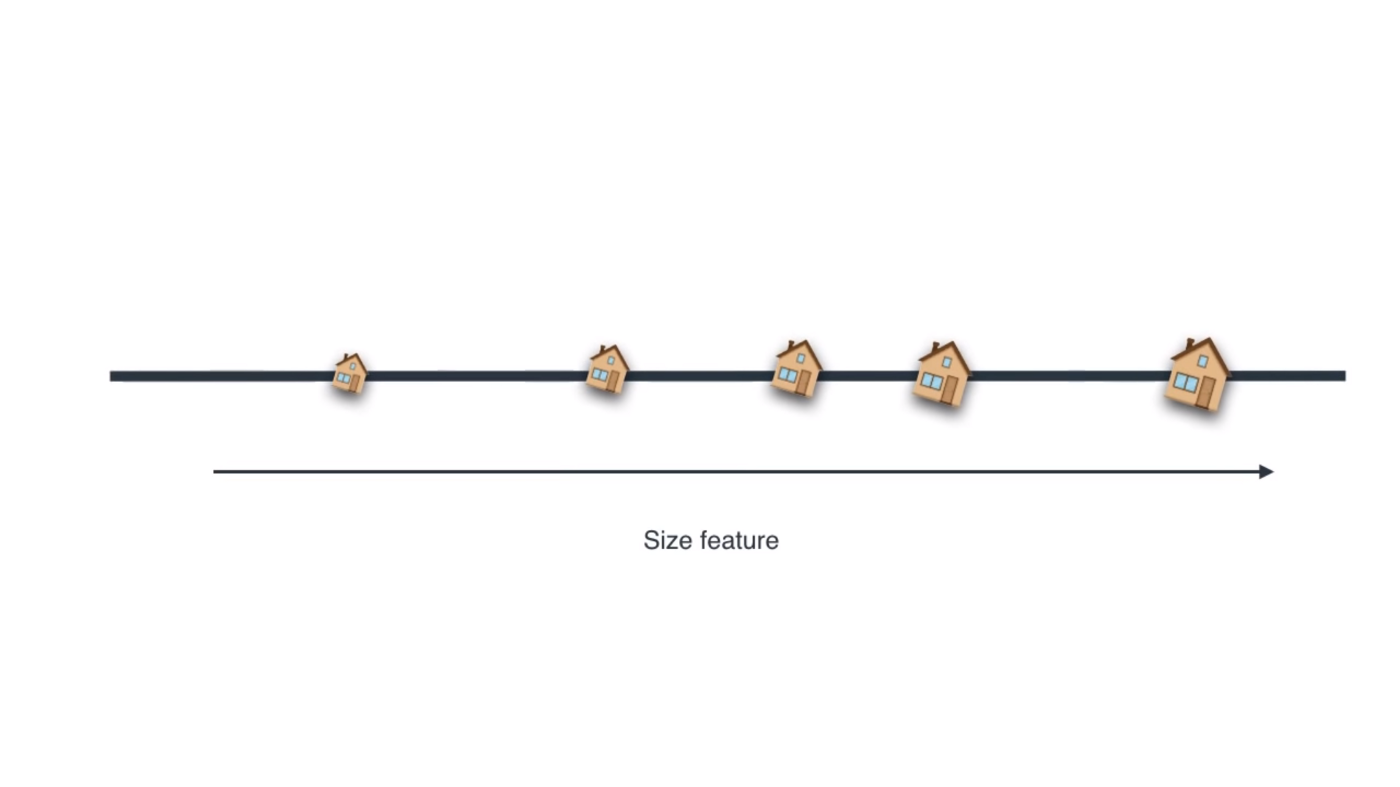
\includegraphics[scale=.25]{figures/pca3}
  \\
  \tiny
\end{figure}


\end{frame}
%----------------------------------------------------------------------%
\begin{frame}
\frametitle{PCA}

\begin{itemize}


\item El primer componente de un conjunto de variables \(X_1,X_2,\dots,X_k\) es
\medskip
\begin{align}
f_1= \delta_{11} x_1+ \delta_{12} x_2 + \dots + \delta_{1k} x_k
\end{align}

\item  \(f_1\) denota al primer componente principal 
\medskip
\item  \(\delta_{ij}\) se conocen como pesos o ``loadings'' del primer componente principal. 
\medskip
\item Esta ecuación ilustra también el hecho de que el primer componente principal es una combinación lineal de las variables
originales. 
\medskip
\pause
\item La pregunta que naturalmente surge es: ¿Cómo se calculan estos componentes de forma tal que preserven la mayor información posible?
\end{itemize}
\end{frame}
%----------------------------------------------------------------------%
\begin{frame}
\frametitle{PCA}
\begin{itemize}
\item La pregunta que naturalmente surge es: ¿Cómo se calculan estos componentes de forma tal que preserven la mayor información posible?

\medskip
\item Formalmente, supongamos que \(X\) es una matriz \(n \times k\) que contiene los datos, es decir, las \(n\) observaciones de las \(k\)
variables.
\medskip
\item  Asumimos que cada una de las variables en \(X\) están centradas para tener media cero. 

\medskip
\item  La matriz \(X\), a su vez, tiene una matriz de covarianza asociada denotada con \(S=Var(X)\), que por definición es una matriz cuadrada de orden \(k\).

\end{itemize}
\end{frame}
%----------------------------------------------------------------------%
\begin{frame}
\frametitle{PCA}
\begin{itemize}

  \item La tarea del primer componente principal es encontrar la combinación lineal de las variables originales que maximiza la varianza, es decir, preservan la mayor información posible. 
  \item El objetivo es crear un índice \(f_1\) que tiene la siguiente forma:
  \medskip
  \begin{align}
  f_1 &= X \delta'_1 \\
      &= \delta_{11} x_1+ \delta_{12} x_2 + \dots + \delta_{1k} x_k
  \end{align}

  \item  El problema consiste en elegir \(\delta_1\) óptimamente, ya que este indice va a ser la ``mejor'' combinación lineal de \(x_1, x_2, \dots, x_k\). 
  \medskip
  \item Definimos como ``mejor'' a aquella combinación lineal que maximiza la varianza. 
  %\item Dicho de otra forma, vamos a buscar maximizar la varianza de forma tal que podamos reproducir de la mejor manera posible la variabilidad (información) original de las variables \(x_j\).
\end{itemize}
\end{frame}
%----------------------------------------------------------------------%
\begin{frame}
\frametitle{PCA}

\begin{itemize}

  \item Notando que

\begin{align}
Var(f_1) &= Var(X \delta'_1) \\
       &= \delta_1 Var(X ) \delta'_1 \\
       &= \delta_1 S \delta'_1 
\end{align}

\item el problema se reduce a elegir \(\delta_1\) de forma que maximice \(Var(X \delta_1)\). 
\pause
\item Maximizar \(\delta_1 S \delta'_1\) tiene como solución trivial llevar \(\delta_1\) a infinito \((\delta_1 \rightarrow \infty)\).
\end{itemize}

\end{frame}
%----------------------------------------------------------------------%
\begin{frame}
\frametitle{PCA}

\begin{itemize}

  \item Para que esta maximización tenga solución en la practica se impone una restricción adicional que normaliza \(\delta_1\):
\medskip
\begin{align}
\delta_1\delta'_1=1
\end{align}

\item Esto restringe a que la suma del cuadrado de los pesos o ``loadings'' sean igual a uno, 
\end{itemize}
\end{frame}
%----------------------------------------------------------------------%
\begin{frame}
\frametitle{PCA}


\begin{itemize}

  \item El problema queda definido de la siguiente manera:
\medskip
\begin{align}
\underset{\delta_1}{max}\,\, \delta_1 S \delta'_1 \\ 
\text{sujeto a}  \\ 
\delta_1 \delta'_1 = 1 
\end{align}
\medskip
\item maximiza \(\delta_1 S \delta'_1\) restringiendo que \(\delta_1\delta'_1=1\). Escribiendo el Lagrangiano,
\medskip
\begin{align}
\mathcal{L} = \delta_1 S \delta'_1 + \lambda_1 (1-\delta_1\delta'_1)
\end{align}
\end{itemize}

\end{frame}
%----------------------------------------------------------------------%
\begin{frame}
\frametitle{PCA}

\begin{itemize}

  \item maximizamos esta expresión de la forma habitual derivando respecto a \(\delta_1\) e igualando a cero:

\begin{align}
\frac{\partial \mathcal{L}}{\partial \delta_1}=S \delta'_1 - \lambda_1 \delta'_1 =0
\end{align}

\item Reordenando:

\begin{align}
S \delta'_1 = \lambda_1 \delta'_1
\end{align}

\item En el óptimo, \(\delta_1\) es el eigenvector correspondiente al eigenvalor \(\lambda\). Premultiplicando la ecuación anterior por
\(\delta_1\) y usando la restricción \(\delta_1\delta'_1=1\):
\end{itemize}


\begin{align}
\delta_1 S \delta'_1 = \lambda_1 
\end{align}

\end{frame}
%----------------------------------------------------------------------%
\begin{frame}
\frametitle{PCA}

\begin{align}
\delta_1 S \delta'_1 = \lambda_1 
\end{align}

\begin{itemize}

\medskip
\item Para maximizar \(\delta_1 S \delta'_1\) debemos elegir \(\lambda_1\) igual al máximo eigenvalor de \(S\) y \(\delta_1\) igual al eigenvalor
correspondiente. 
\medskip
\item  Notando además que \(\delta_1 S \delta'_1=Var(X \delta'_1)\), el problema de encontrar la mejor combinación lineal que reproduce la variabilidad en \(X\) se reduce a encontrar el mayor eigenvalor de \(S\) y su correspondiente eigenvector.

\end{itemize}


\end{frame}
%----------------------------------------------------------------------%
\begin{frame}
\frametitle{PCA}

\begin{itemize}


\item Luego de calcular el primer componente principal \(f_1\), 
\medskip
\item podemos encontrar también el segundo componente principal, \(f_2\):

\begin{align}
f_2 &= X \delta'_2 \\ 
    &= \delta_{21} x_1+ \delta_{22} x_2 + \dots + \delta_{2k} x_k
\end{align}

\item El segundo componente principal, será la combinación lineal que tiene la máxima varianza de todas las combinaciones lineales ortogonales a
\(f_1\).
\medskip
\item En otras palabras, responde a la pregunta: ¿Cuál es la mejor combinación lineal de las variables \(x_1,x_2,\dots,x_k\) no correlacionada al primer componente principal? 
\medskip
\item Intuitivamente, esta es la ``segunda mejor'' combinación lineal de \(x_1,x_2,\dots,x_k\), que no esta contenida en el primer componente.
\end{itemize}
\end{frame}
%----------------------------------------------------------------------%
\begin{frame}
\frametitle{PCA}

El cálculo del segundo componente entonces responde al siguiente
problema:

\begin{align}
\underset{\delta_2}{max}\,\, \delta_2 S \delta'_2 \\
\text{sujeto a}   \\
\delta_2 \delta'_2 &= 1   \\
y \\ 
\delta_2 \delta'_1 &=0 \\ \nonumber
\end{align}

\end{frame}
%----------------------------------------------------------------------%
\begin{frame}
\frametitle{PCA}

\begin{itemize}
\item La solución  es el eigenvector asociado al segundo eigenvalor mas grande.
\medskip
\item Siguiendo esta lógica, por inducción es posible seguir calculando componentes cada uno ortogonal entre si y decrecientes en importancia.
\medskip
\item En general, para una matriz \(X\) con \(n\) observaciones y \(k\) variables tiene al menos el mínimo entre el número de observaciones
menos 1 \((n-1)\) y el número de variables \((k)\), componentes principales distintos.

\begin{align}
\#PC= (min(n-1,k)
\end{align}

\end{itemize}



\end{frame}
%----------------------------------------------------------------------%
\subsection{Aspectos Operativos}
%----------------------------------------------------------------------%
\begin{frame}
\frametitle{Escalar las variables}



\begin{itemize}
 \item  Desde un punto estrictamente matemático no hay nada intrínsecamente incorrecto en hacer combinaciones lineales de variables con diferentes unidades de medida. 
\medskip
 \item Sin embargo, cuando usamos PCA buscamos maximizar varianza y la varianza se ve
afectada por las unidades de medida.

\item  Esto implica que los componentes principales basados en la matriz de covarianza \(S\) van a cambiar si las unidades de medida de una o más variables cambian. 
\item Para que esto no suceda, es práctica habitual estandarizar las variables. Es decir, cada
valor de \(X\) es recentrado y dividido por la desviación estándar:

\begin{align}
  z_{ij} = \frac{x_{ij}-\bar{x_j}}{s_j}
\end{align}

 \end{itemize}

\end{frame}
%----------------------------------------------------------------------%
\begin{frame}
\frametitle{Descomposición espectral}


\begin{itemize}


\item La descomposición espectral o eigendecomposición es una forma de descomponer matrices. 
\medskip
\item Descomponer una matriz significa que queremos encontrar un producto de matrices que sea igual a la matriz inicial. 
\medskip
\item En el caso de la eigendecomposición, descomponemos la matriz inicial en el producto de sus eigenvectores y eigenvalores.


 \end{itemize}

\end{frame}
%----------------------------------------------------------------------%
\begin{frame}
\frametitle{Descomposición espectral}


\begin{itemize}

\item Veamos cómo se usan los eigenvectores y eigenvalores para descomponer una matriz. 
\medskip
\item Tomando los eigenvectores de una matriz \(A_{m\times m}\) podemos concatenarlos y colocarlos en una matriz \(P\).
\medskip
\item  Entonces \(P\) será una matriz cuyas columnas son los eigenvectores de \(A\):

\begin{align}
A= P\Lambda P'
\end{align}

\item donde \(\Lambda =diag(\lambda)\) es una matriz diagonal de los eigenvalores.
\medskip
\item Es importante notar que esta descomposición sólo es válida para matrices cuadradas, como lo es la matriz de covarianza. Por lo tanto, no puede ser utilizada para matrices no cuadradas.
\end{itemize}
\end{frame}

%----------------------------------------------------------------------%
\begin{frame}
\frametitle{Proporción de Varianza Explicada}

\begin{itemize}


\item Una propiedad muy útil del procedimiento del cálculo de componentes  principales es que la variabilidad total de \(X\) es la suma de los
 \(k\) eigenvalores de \(V(X)=S\). 
 \item Para demostrarlo supongamos que \(\lambda_1,\dots,\lambda_k\) son los eigenvalores de \(V(X)=S\),  ordenados de mayor a menor, 
 \item  \(p_1 , \dots , p_K\) son los  eigenvectores correspondientes. 
 \item Adicionalmente llamemos \(P\) a la  matriz cuyas columnas son estos eigenvectores.

\end{itemize}
\end{frame}

%----------------------------------------------------------------------%
\begin{frame}
\frametitle{Proporción de Varianza Explicada}

\begin{itemize}
\item  Supongamos también que \(f_j= X \delta'_j\) es el \(j-esimo\)  componente principal, entonces

\begin{align}
V (f_j ) &= \delta_j S \delta'_j  \\\
         &= p_j P\Lambda P' p'_j  \\\
         &= \lambda_j
\end{align}



\item Este resultado nos dices que la varianza del \(j-esimo\) componente  principal es el \(j-esimo\) eigenvalor ordenado de S.

\item  Usando este resultado podemos ver que la varianza total de \(X\) va a
% ser la suma de las varianza de las variables \(x_j\):


\end{itemize}
\end{frame}

%----------------------------------------------------------------------%
\begin{frame}
\frametitle{Proporción de Varianza Explicada}

\begin{itemize}


\item Entonces

\begin{align}
tr(\Sigma) = tr(P \Lambda P')= tr(PP' \Lambda ) = \sum_{j=1}^k \lambda_j= \sum_{j=1}^k V(f_j)
\end{align}

\item Este resultado nos permite preguntarnos: ¿Cuánta información perdimos por proyectar los datos en unos cuantos componentes principales? 
\medskip
\item ¿Cuánto de la varianza esta contenida en los primeros componentes
principales? 


\begin{align}
\frac{\lambda_k}{\sum_{j=1}^k \lambda_j}
\end{align}
\end{itemize}

\end{frame}
%----------------------------------------------------------------------%
\begin{frame}
\frametitle{¿Cuántos componentes principales debemos seleccionar?}

\begin{itemize}
\item Mencionamos que una matriz $X$ de dimensión $(n \times k)$ tiene en general $min(n-1,k)$ componentes principales distintos.
\medskip
 \item En la práctica generalmente no estamos interesados en todos los componentes, sino más bien quedarnos con los primeros que nos permitan visualizar o interpretar datos. 
\medskip
\item En efecto, nos gustaría quedarnos con el mínimo numero que nos permita una buena comprensión de los datos. 
\medskip
\end{itemize}

\end{frame}
%----------------------------------------------------------------------%
\begin{frame}
\frametitle{¿Cuántos componentes principales debemos seleccionar?}

\begin{itemize}
 \item La pregunta natural que surge aquí es si hay una forma establecida para determinar el número de componentes principales a utilizar.
 \medskip
 \item  Desafortunadamente, no existe una forma objetiva aceptada en la literatura de responderla. Sin embargo, hay tres enfoques simples que pueden servir de guía para decidir el número de componentes principales relevantes.

Estos son:

  \begin{itemize}

    \item Examen visual de un gráfico de sedimentación (scree plot).
    \item Proporción de varianza explicada.
    \item Criterio de Kaiser.
  \end{itemize}
\end{itemize}

\end{frame}
%----------------------------------------------------------------------%

%----------------------------------------------------------------------%
\begin{frame}
\frametitle{Examen visual de un gráfico de sedimentación (screeplot)}
    


\begin{figure}[H] \centering

    \centering
    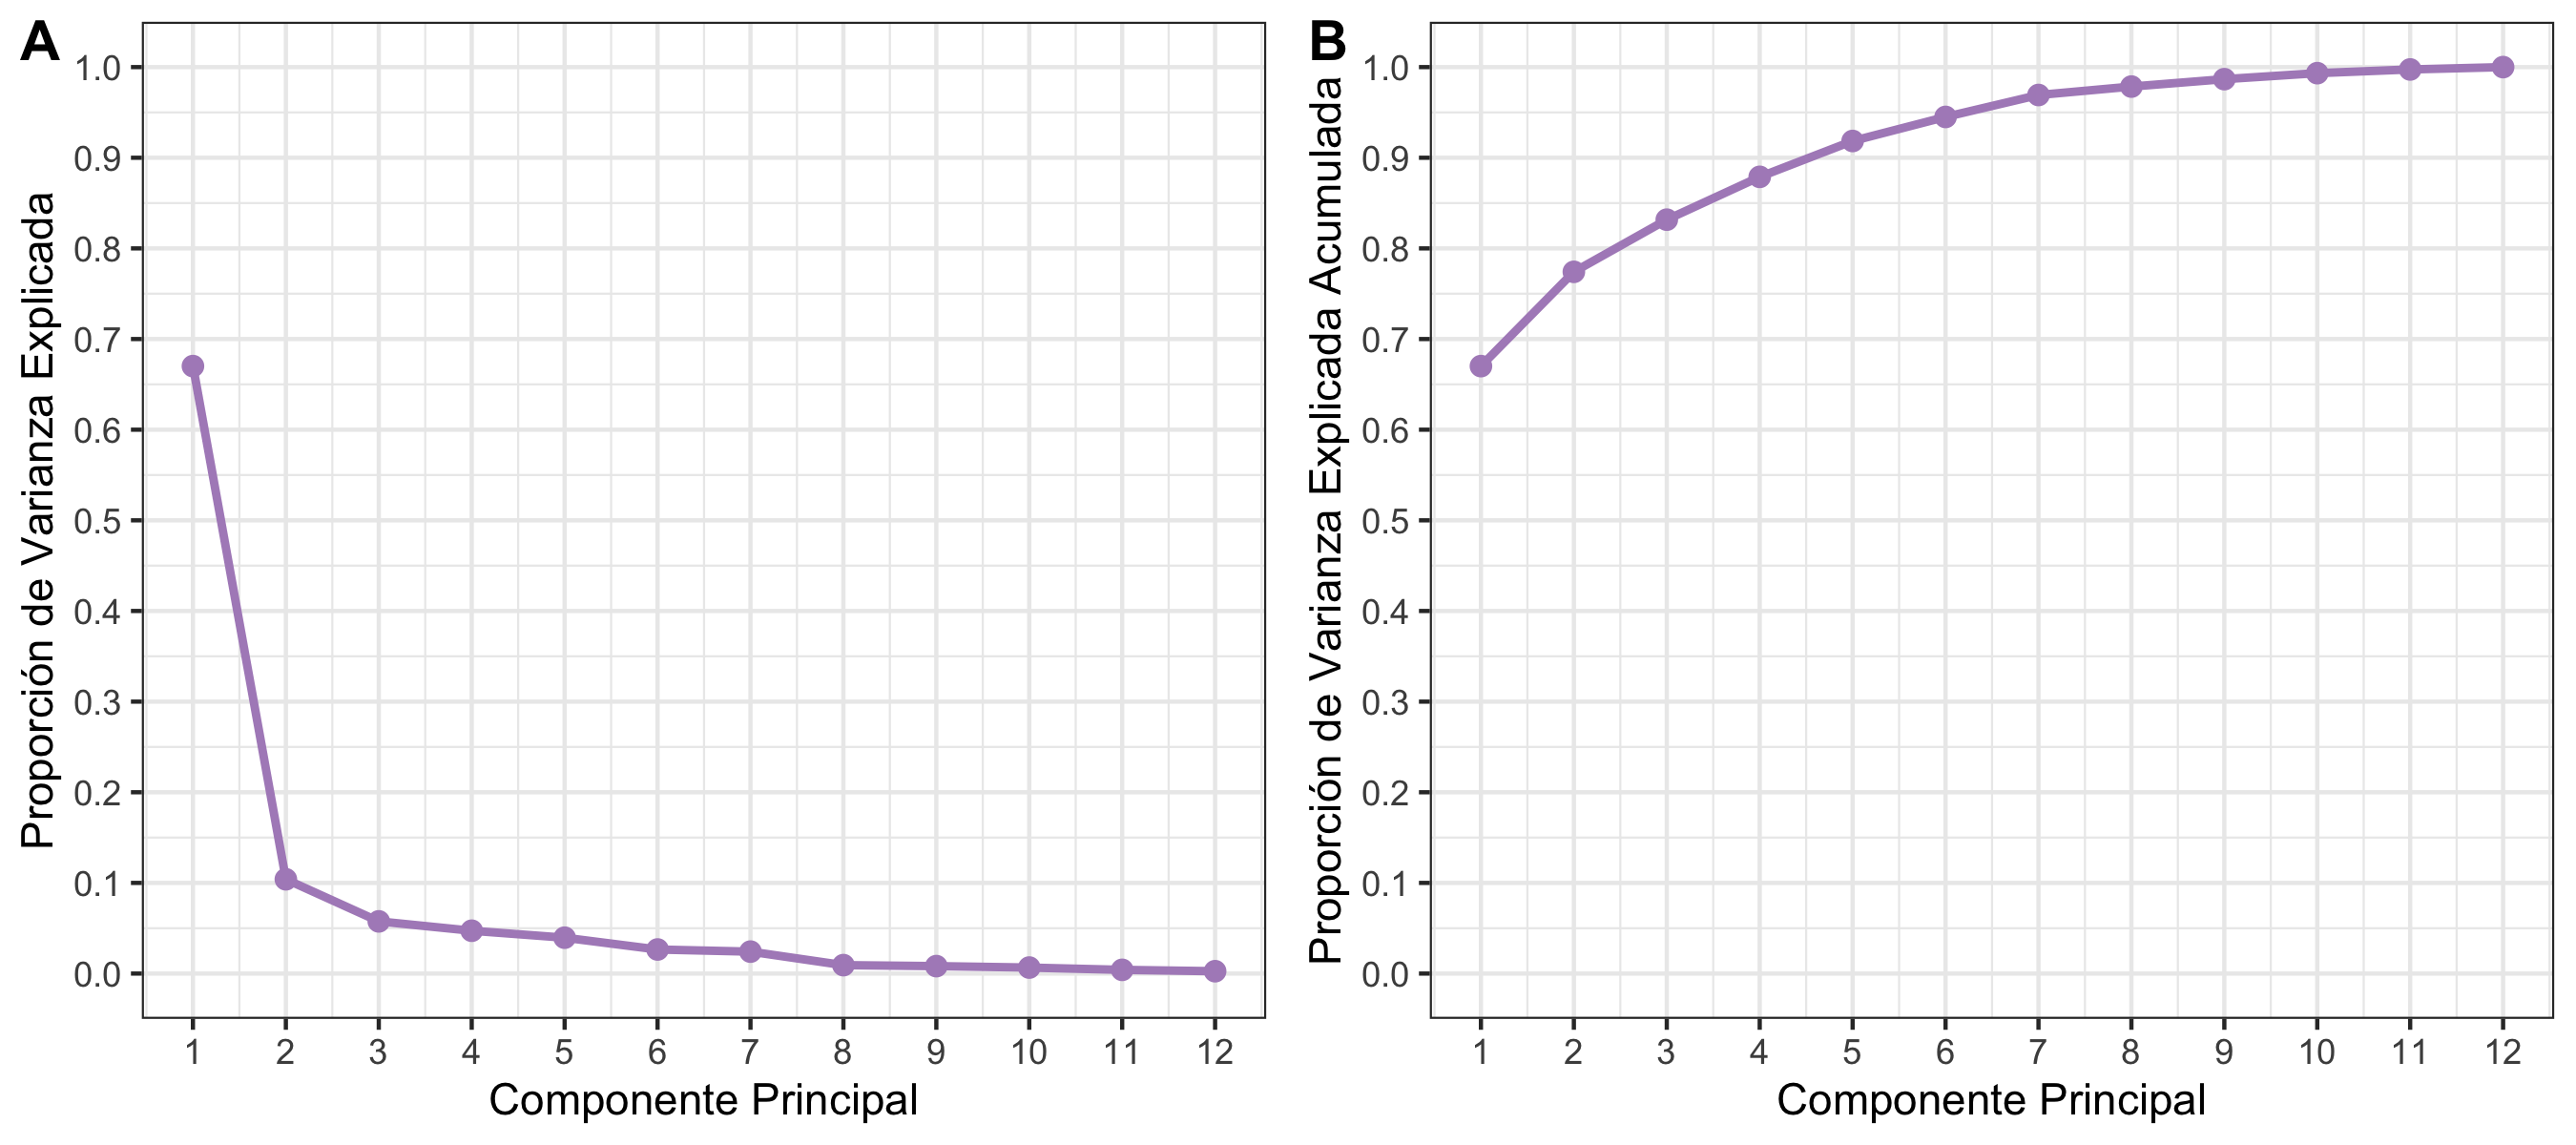
\includegraphics[scale=.1]{figures/plot_S1_LSC2_1.png}
  \\
  \tiny
\end{figure}


\end{frame}

%----------------------------------------------------------------------%
\begin{frame}
\frametitle{Proporción de varianza explicada}


\begin{itemize}


  \item Otro enfoque a menudo utilizado en la práctica, es imponer un umbral a priori y elegir los componentes principales en base a esta.
  \medskip
  \item  Por ejemplo podríamos definir un umbral del 90\%, o 70\%
  \medskip
  \item El umbral a definir dependerá de la aplicación, el contexto, y el conjunto de los datos. 
  \medskip
  \item Típicamente se utilizan umbrales entre el 70\% y el 90\%.
\end{itemize}
\end{frame}

%----------------------------------------------------------------------%
\begin{frame}
\frametitle{Criterio de Kaiser}

\begin{itemize}


\item El criterio de Kaiser es otro enfoque ampliamente utilizado para evaluar el número máximo de componentes principales. 
\medskip
\item Este sugiere que solo se retengan los componentes principales cuyos eigenvalores sean mayores a 1. 
\medskip
\item La idea es que se retengan aquellos componentes cuyos eigenvalues sean superiores a la media de los eigenvalues:

\begin{align}
\lambda_h> \frac{\sum_j^k \lambda_j}{k}
\end{align}

\medskip
\item Dado que los datos están estandarizados tenemos que \(\sum_j^k \lambda_j=k\), por lo que es equivalente a buscar los eigenvalues mayores a uno.
\end{itemize}
\end{frame}

%----------------------------------------------------------------------%
\section{Clusters}
%----------------------------------------------------------------------%
\begin{frame}[fragile]
\frametitle{}


\centering
{\huge \textcolor{andesred}{Clusters}}



\end{frame}
%----------------------------------------------------------------------%
\begin{frame}
\frametitle{Análisis de Clusters}


\begin{itemize}

  \item El análisis de clústeres (también llamado segmentación de datos) es una de las principales aplicaciones de los algoritmos de aprendizaje no
  supervisado 
  \medskip
  \item consiste dividir las observaciones de un conjunto en un número \(m\) de grupos de tal manera que todos los puntos dentro de un mismo grupo estén más estrechamente relacionados entre sí que los puntos asignados a diferentes grupos.
  \medskip
  \item un concepto central en todo análisis de clústeres es la noción de similaridad o disimilaridad entre observaciones la cual podrá variar
  según las decisiones del investigador. 
  \medskip
  \item Existen algunas guías para escoger una adecuada medida de distancia, sin embargo, existe un buen grado de subjetividad 
\end{itemize}

\end{frame}
%----------------------------------------------------------------------%
\subsection{Medidas de distancia o disimilaridad}

%----------------------------------------------------------------------%
\begin{frame}
\frametitle{Matrices de distancia o disimilaridad}

\begin{itemize}
\item Muchas veces los datos son presentados directamente en términos de proximidad entre pares de objetos. 
\medskip
\item Este tipo de datos generalmente se representa en una matriz \(D\) de tamaño \(N\times N\) en donde \(N\) es el número de objetos y cada elemento \(d_{ij}\) corresponde a la proximidad entre el objeto \(i\) y el objeto \(j\).
\medskip
\item  En muchos casos esta matriz se usa como insumo en los algoritmos de clustering.
\medskip
\item La mayoría de algoritmos suponen que la matriz de disimilaridad debe ser no negativa y con ceros en la diagonal (es decir que la distancia de un
objeto a si mismo es 0). 
\end{itemize}






\end{frame}
%----------------------------------------------------------------------%
\begin{frame}
\frametitle{Distancia}

\begin{itemize}


\item Entre las medidas de distancia más comunes se encuentra la distancia euclideana: 
\begin{align}
d_j(x_{ij}, x_{i'j}) = (x_{ij} - x_{i'j})^2
\end{align}

\item Muy útil para variables continuas
\medskip
\item Para atributos no cuantitativos (como las variables categóricas) la distancia al cuadrado no es apropiada. 

\end{itemize}

\end{frame}
%----------------------------------------------------------------------%
\begin{frame}
\frametitle{Distancia}

\begin{itemize}


\item Para variables cuantitativas es usual definir el error entre ellas como una función monótona creciente del valor absoluto de su diferencia:
\begin{align}
d(x_i, x_{i'})=l(|x_i, x_{i'}|)
\end{align}

\medskip
\item Para variables ordinales: Este tipo de variables usualmente se representa como un continuo de enteros y el dominio de estos es considerado un conjunto ordenado. 

\medskip
$\frac{i-1/2}{M},\ i=1,\cdots,M$ 

\medskip
\item En el orden prescrito de sus valores originales. Luego se tratan como variables cuantitativas en esta escala.

\end{itemize}

\end{frame}
%----------------------------------------------------------------------%
\subsection{K-Medias}
%----------------------------------------------------------------------%
\begin{frame}[fragile]
\frametitle{}


\centering
{\huge \textcolor{andesred}{K-Medias}}



\end{frame}
%----------------------------------------------------------------------%
\begin{frame}
\frametitle{K-Medias}


\begin{itemize}
  \item K-Medias es quizas el algoritmo mas conocido para hacer agrupamiento
\medskip
\item Es un algoritmo de descenso iterativo. 
\medskip
\item Este se usa cuando todas las variables en el conjunto de datos son numéricas y se utiliza la distancia euclidiana cuadrática para definir la disimilaridad entre observaciones:
\medskip
\begin{align}
d(x_i, x_{i'})=\sum_{j=1}^p(x_{ij}-x_{i'j})^2=||x_i-x_{i'}||^2 
\end{align}
\end{itemize}



\end{frame}
%----------------------------------------------------------------------%
\begin{frame}
\frametitle{K-Medias}


\begin{itemize}

\item En este caso particular la función de pérdida a minimizar para garantizar que los puntos más cercanos entre sí estén dentro de un mismo segmento
es:

\begin{align}
W(C) &= \frac{1}{2}\sum_{k=1}^K\sum_{C(i)=k}\sum_{C(i')=k}||x_i-x_{i'}||^2 \\
     &= \sum_{k=1}^K N_k\sum_{C(i)=k}||x_i-\bar{x_{k}}||^2 
\end{align}



\item En donde \(\bar{x_{k}}=(\bar{x_{1k}}, \cdots, \bar{x_{pk}})\) es el vector de
medias asociado al clúster k-ésimo y \(N_k=\sum_{i=1}^N(C(i)=k)\). 


\end{itemize}



\end{frame}
%----------------------------------------------------------------------%
\begin{frame}
\frametitle{K-Medias}

\begin{itemize}


\item Para minimizar la expresión pasada se usa el siguiente algoritmo: 
\begin{enumerate}
  \item Para una determinada asignación de clusters $K$, la varianza total de los conglomerados se minimiza con respecto a $\{m_1, \cdots , m_K\}$ obteniendo las medias de los clusters asignados actualmente $\bar{x_s}=argmin_m \sum_{i\in S} ||x_i - m||^2$. 
  \medskip
  \item Dado un conjunto actual de medias $\{m_1, \cdots , m_K\}$, la varianza total de los conglomerados se minimiza asignando cada observación a la media del conglomerado más cercana. Es decir, \[C(i)=argmin_{1\leq k \leq K} ||x_i-m_k||^2\] 
  \medskip
  \item Se repiten los pasos 1 y 2 hasta que las asignaciones no cambien.
\end{enumerate}

\end{itemize}

\end{frame}
%----------------------------------------------------------------------%
\begin{frame}
\frametitle{Aspectos operativos}
\framesubtitle{Gráfica de Codo}



\begin{figure}[H] \centering

    \centering
    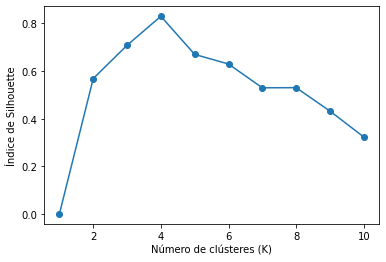
\includegraphics[scale=.7]{figures/output_36_0.png}
  \\
  \tiny
\end{figure}



\end{frame}
%----------------------------------------------------------------------%
\begin{frame}
\frametitle{Aspectos operativos}
\framesubtitle{Coeficiente de Silhouette}

\begin{figure}[H] \centering

    \centering
    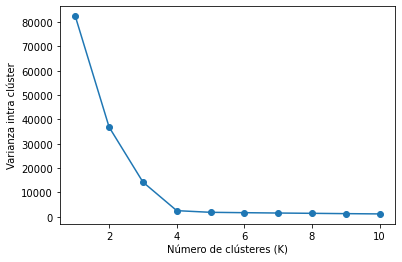
\includegraphics[scale=.7]{figures/output_35_0.png}
  \\
  \tiny
\end{figure}
\end{frame}
%----------------------------------------------------------------------%
\begin{frame}
\frametitle{Aspectos operativos}

\begin{itemize}
\item Cada uno de los pasos 1 y 2 reduce el valor de la varianza total de los conglomerados, por lo que la convergencia está asegurada.
\medskip
 \item Sin embargo, el resultado puede representar un mínimo local subóptimo. 

 \medskip
 \item Por ende se recomienda iniciar el algoritmo con varias opciones aleatorias diferentes para las medias iniciales y elegir la solución que tenga el
valor más pequeño de la función objetivo.
\end{itemize}
\end{frame}   
%----------------------------------------------------------------------%
\begin{frame}
\frametitle{Ejemplo}
\framesubtitle{Simulación}


\begin{figure}[H] \centering

    \centering
    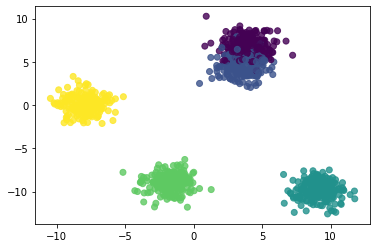
\includegraphics[scale=.7]{figures/cl_teoricos1.png}
  \\
  \tiny
\end{figure}


\end{frame}
%----------------------------------------------------------------------%
\begin{frame}
\frametitle{Ejemplo}
\framesubtitle{Observamos}


\begin{figure}[H] \centering

    \centering
    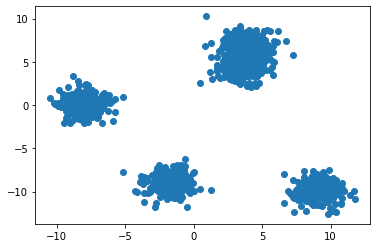
\includegraphics[scale=.7]{figures/cl_teoricos2.png}
  \\
  \tiny
\end{figure}


\end{frame}
%----------------------------------------------------------------------%
\begin{frame}
\frametitle{Ejemplo}
\framesubtitle{Proceso K=2}


\begin{figure}[H] \centering

    \centering
    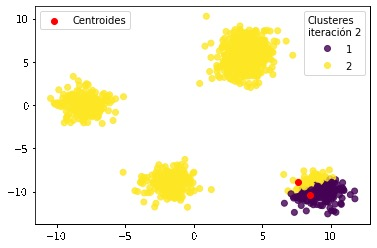
\includegraphics[scale=.7]{figures/k2_1.jpg}
  \\
  \tiny
\end{figure}


\end{frame}
%----------------------------------------------------------------------%
\begin{frame}
\frametitle{Ejemplo}
\framesubtitle{Proceso K=2}


\begin{figure}[H] \centering

    \centering
    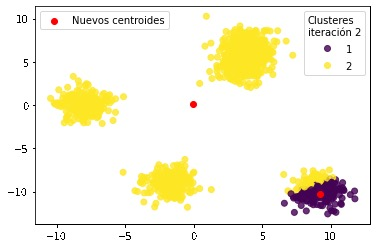
\includegraphics[scale=.7]{figures/k2_2.jpg}
  \\
  \tiny
\end{figure}



\end{frame}
%----------------------------------------------------------------------%
\begin{frame}
\frametitle{Ejemplo}
\framesubtitle{Proceso K=2}


\begin{figure}[H] \centering

    \centering
    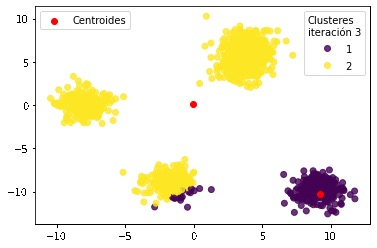
\includegraphics[scale=.7]{figures/k2_3.jpg}
  \\
  \tiny
\end{figure}


\end{frame}
%----------------------------------------------------------------------%
\begin{frame}
\frametitle{Ejemplo}
\framesubtitle{Proceso K=2}


\begin{figure}[H] \centering

    \centering
    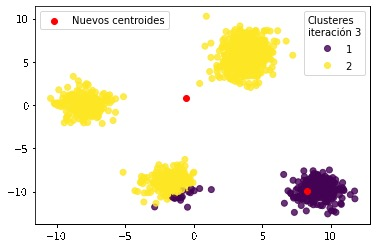
\includegraphics[scale=.7]{figures/k2_4.jpg}
  \\
  \tiny
\end{figure}


\end{frame}
%----------------------------------------------------------------------%
\begin{frame}
\frametitle{Ejemplo}
\framesubtitle{Proceso K=2}


\begin{figure}[H] \centering

    \centering
    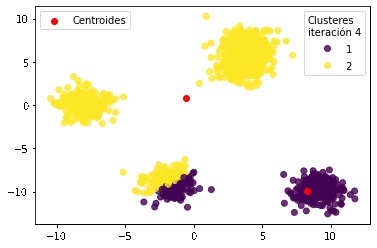
\includegraphics[scale=.7]{figures/k2_5.jpg}
  \\
  \tiny
\end{figure}


\end{frame}
%----------------------------------------------------------------------%
\begin{frame}
\frametitle{Ejemplo}
\framesubtitle{Proceso K=2}


\begin{figure}[H] \centering

    \centering
    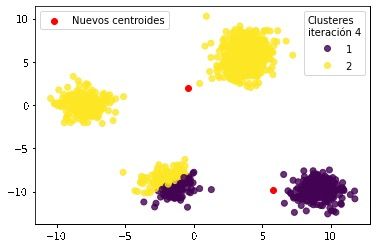
\includegraphics[scale=.7]{figures/k2_6.jpg}
  \\
  \tiny
\end{figure}


\end{frame}
%----------------------------------------------------------------------%
\begin{frame}
\frametitle{Ejemplo}
\framesubtitle{Proceso K=2}


\begin{figure}[H] \centering

    \centering
    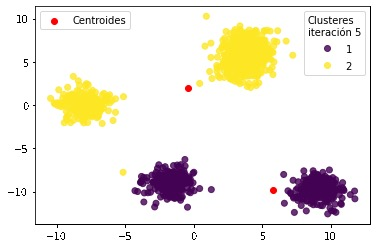
\includegraphics[scale=.7]{figures/k2_7.jpg}
  \\
  \tiny
\end{figure}


\end{frame}
%----------------------------------------------------------------------%
\begin{frame}
\frametitle{Ejemplo}
\framesubtitle{Proceso K=2}


\begin{figure}[H] \centering

    \centering
    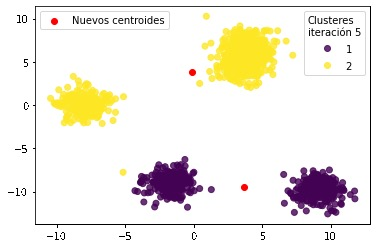
\includegraphics[scale=.7]{figures/k2_8.jpg}
  \\
  \tiny
\end{figure}



\end{frame}
%----------------------------------------------------------------------%
\begin{frame}
\frametitle{Ejemplo}
\framesubtitle{Proceso K=2}


\begin{figure}[H] \centering

    \centering
    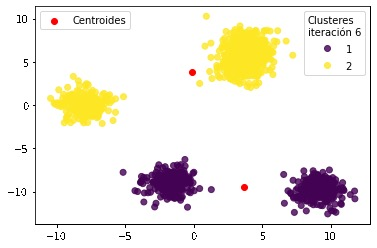
\includegraphics[scale=.7]{figures/k2_9.jpg}
  \\
  \tiny
\end{figure}



\end{frame}
%----------------------------------------------------------------------%
\begin{frame}
\frametitle{Ejemplo}
\framesubtitle{Proceso K=2}


\begin{figure}[H] \centering

    \centering
    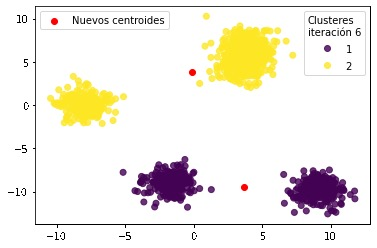
\includegraphics[scale=.7]{figures/k2_10.jpg}
  \\
  \tiny
\end{figure}


\end{frame}
%----------------------------------------------------------------------%
\begin{frame}
\frametitle{Ejemplo}
\framesubtitle{Proceso K=2}


\begin{figure}[H] \centering

    \centering
    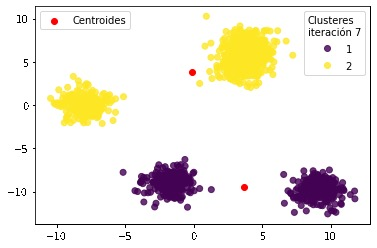
\includegraphics[scale=.7]{figures/k2_11.jpg}
  \\
  \tiny
\end{figure}


\end{frame}
%----------------------------------------------------------------------%
\begin{frame}
\frametitle{Ejemplo}
\framesubtitle{Proceso K=2}


\begin{figure}[H] \centering

    \centering
    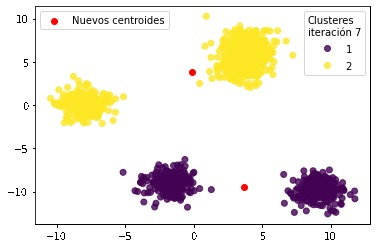
\includegraphics[scale=.7]{figures/k2_12.jpg}
  \\
  \tiny
\end{figure}


\end{frame}
%----------------------------------------------------------------------%
\begin{frame}
\frametitle{Ejemplo}
\framesubtitle{Proceso K=4}


\begin{figure}[H] \centering

    \centering
    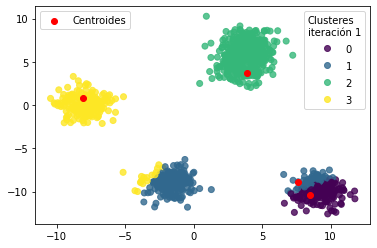
\includegraphics[scale=.7]{figures/output_12_0.png}
  \\
  \tiny
\end{figure}

\end{frame}
%----------------------------------------------------------------------%
\begin{frame}
\frametitle{Ejemplo}
\framesubtitle{Motivación}


\begin{figure}[H] \centering

    \centering
    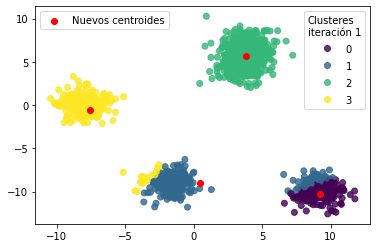
\includegraphics[scale=.7]{figures/output_16_0.png}
  \\
  \tiny
\end{figure}


\end{frame}
%----------------------------------------------------------------------%
\begin{frame}
\frametitle{Ejemplo}
\framesubtitle{Motivación}


\begin{figure}[H] \centering

    \centering
    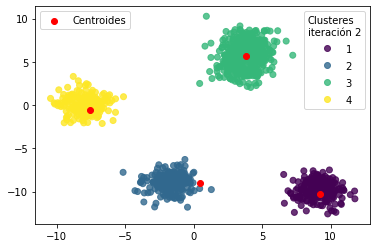
\includegraphics[scale=.7]{figures/output_17_1.png}
  \\
  \tiny
\end{figure}

\end{frame}
%----------------------------------------------------------------------%
\begin{frame}
\frametitle{Ejemplo}
\framesubtitle{Motivación}


\begin{figure}[H] \centering

    \centering
    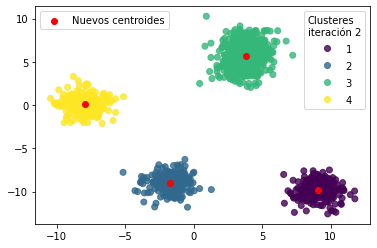
\includegraphics[scale=.7]{figures/output_17_2.png}
  \\
  \tiny
\end{figure}

\end{frame}
%----------------------------------------------------------------------%
\begin{frame}
\frametitle{Ejemplo}
\framesubtitle{Motivación}


\begin{figure}[H] \centering

    \centering
    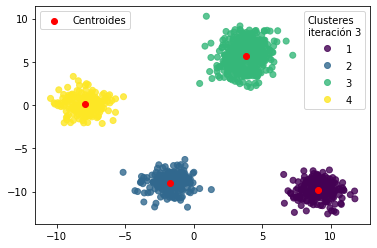
\includegraphics[scale=.7]{figures/output_17_4.png}
  \\
  \tiny
\end{figure}

\end{frame}
%----------------------------------------------------------------------%
\begin{frame}
\frametitle{Ejemplo}
\framesubtitle{Motivación}


\begin{figure}[H] \centering

    \centering
    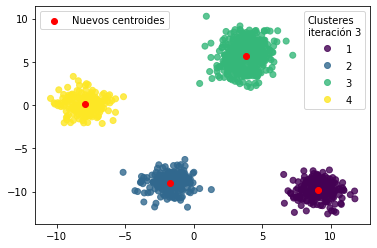
\includegraphics[scale=.7]{figures/output_17_5.png}
  \\
  \tiny
\end{figure}



\end{frame}
%----------------------------------------------------------------------%
\begin{frame}
\frametitle{Ejemplo}
\framesubtitle{Proceso K=5}


\begin{figure}[H] \centering

    \centering
    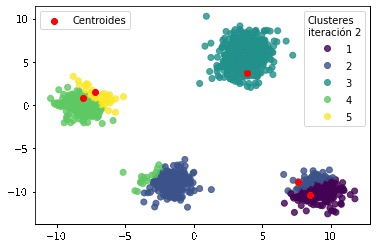
\includegraphics[scale=.7]{figures/k5_1.jpg}
  \\
  \tiny
\end{figure}



\end{frame}
%----------------------------------------------------------------------%
\begin{frame}
\frametitle{Ejemplo}
\framesubtitle{Proceso K=5}


\begin{figure}[H] \centering

    \centering
    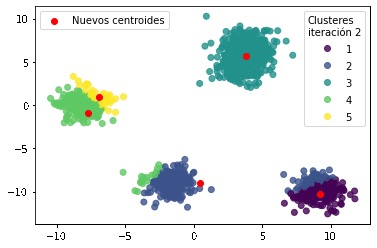
\includegraphics[scale=.7]{figures/k5_2.jpg}
  \\
  \tiny
\end{figure}



\end{frame}
%----------------------------------------------------------------------%
\begin{frame}
\frametitle{Ejemplo}
\framesubtitle{Proceso K=5}


\begin{figure}[H] \centering

    \centering
    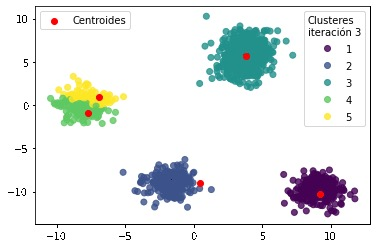
\includegraphics[scale=.7]{figures/k5_3.jpg}
  \\
  \tiny
\end{figure}


\end{frame}
%----------------------------------------------------------------------%
\begin{frame}
\frametitle{Ejemplo}
\framesubtitle{Proceso K=5}


\begin{figure}[H] \centering

    \centering
    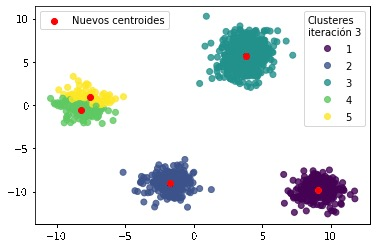
\includegraphics[scale=.7]{figures/k5_4.jpg}
  \\
  \tiny
\end{figure}


\end{frame}
%----------------------------------------------------------------------%
\begin{frame}
\frametitle{Ejemplo}
\framesubtitle{Proceso K=5}


\begin{figure}[H] \centering

    \centering
    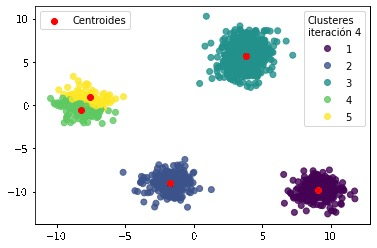
\includegraphics[scale=.7]{figures/k5_5.jpg}
  \\
  \tiny
\end{figure}


\end{frame}
%----------------------------------------------------------------------%
\begin{frame}
\frametitle{Ejemplo}
\framesubtitle{Proceso K=5}


\begin{figure}[H] \centering

    \centering
    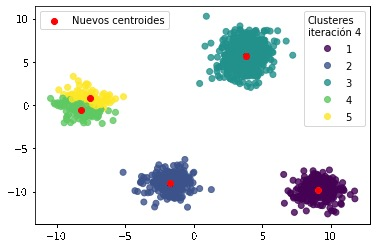
\includegraphics[scale=.7]{figures/k5_6.jpg}
  \\
  \tiny
\end{figure}


\end{frame}
%----------------------------------------------------------------------%
\begin{frame}
\frametitle{Ejemplo}
\framesubtitle{Proceso K=5}


\begin{figure}[H] \centering

    \centering
    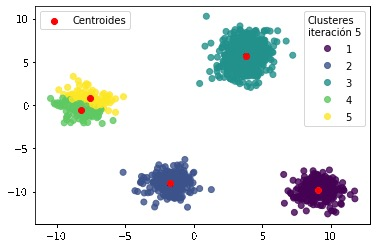
\includegraphics[scale=.7]{figures/k5_7.jpg}
  \\
  \tiny
\end{figure}


\end{frame}
%----------------------------------------------------------------------%
\begin{frame}
\frametitle{Ejemplo}
\framesubtitle{Proceso K=5}


\begin{figure}[H] \centering

    \centering
    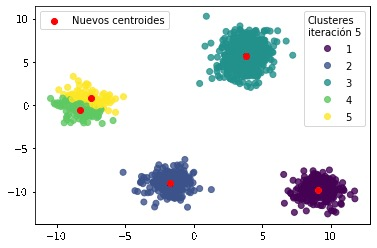
\includegraphics[scale=.7]{figures/k5_8.jpg}
  \\
  \tiny
\end{figure}


\end{frame}
%----------------------------------------------------------------------%
\begin{frame}
\frametitle{Ejemplo}
\framesubtitle{Proceso K=5}


\begin{figure}[H] \centering

    \centering
    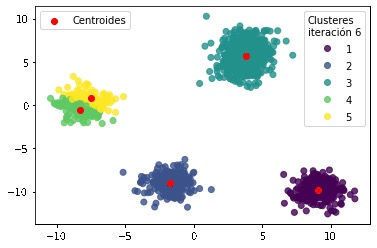
\includegraphics[scale=.7]{figures/k5_9.jpg}
  \\
  \tiny
\end{figure}


\end{frame}
%----------------------------------------------------------------------%
\begin{frame}
\frametitle{Ejemplo}
\framesubtitle{Proceso K=5}


\begin{figure}[H] \centering

    \centering
    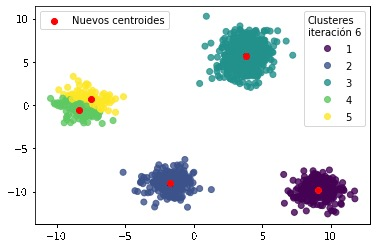
\includegraphics[scale=.7]{figures/k5_10.jpg}
  \\
  \tiny
\end{figure}


\end{frame}
%----------------------------------------------------------------------%
\begin{frame}
\frametitle{Ejemplo}
\framesubtitle{Proceso K=5}


\begin{figure}[H] \centering

    \centering
    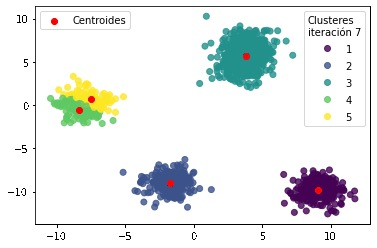
\includegraphics[scale=.7]{figures/k5_11.jpg}
  \\
  \tiny
\end{figure}


\end{frame}
%----------------------------------------------------------------------%
\begin{frame}
\frametitle{Ejemplo}
\framesubtitle{Proceso K=5}


\begin{figure}[H] \centering

    \centering
    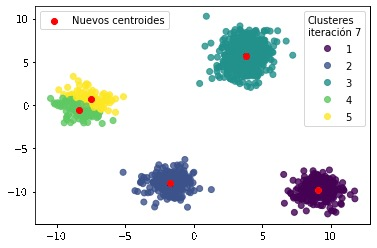
\includegraphics[scale=.7]{figures/k5_12.jpg}
  \\
  \tiny
\end{figure}


\end{frame}
%----------------------------------------------------------------------%
\begin{frame}
\frametitle{Ejemplo}
\framesubtitle{Proceso K=5}


\begin{figure}[H] \centering

    \centering
    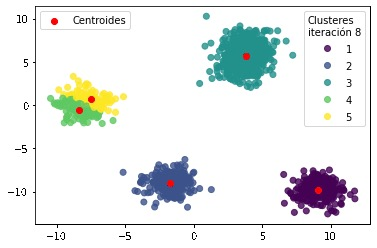
\includegraphics[scale=.7]{figures/k5_13.jpg}
  \\
  \tiny
\end{figure}


\end{frame}
%----------------------------------------------------------------------%
\begin{frame}
\frametitle{Ejemplo}
\framesubtitle{Proceso K=5}


\begin{figure}[H] \centering

    \centering
    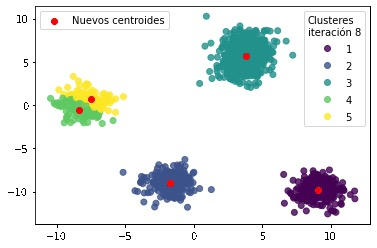
\includegraphics[scale=.7]{figures/k5_14.jpg}
  \\
  \tiny
\end{figure}


\end{frame}
%----------------------------------------------------------------------%
\begin{frame}
\frametitle{Ejemplo}
\framesubtitle{Proceso K=5}


\begin{figure}[H] \centering

    \centering
    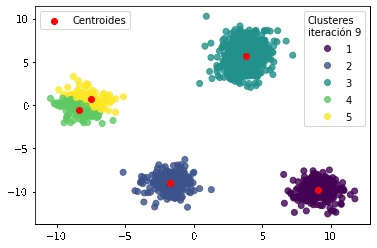
\includegraphics[scale=.7]{figures/k5_15.jpg}
  \\
  \tiny
\end{figure}


\end{frame}
%----------------------------------------------------------------------%
\begin{frame}
\frametitle{Ejemplo}
\framesubtitle{Proceso K=5}


\begin{figure}[H] \centering

    \centering
    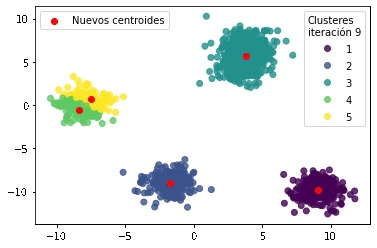
\includegraphics[scale=.7]{figures/k5_16.jpg}
  \\
  \tiny
\end{figure}


\end{frame}

%----------------------------------------------------------------------%
\section{Break}
\begin{frame}
\frametitle{}

\begin{centering}
\huge
\textcolor{andesred}{Volvemos en 15 mins con \texttt{R} }

\end{centering}

\end{frame}
%----------------------------------------------------------------------%
\section{\texttt{R para ML}}
%----------------------------------------------------------------------%
\begin{frame}
\frametitle{R para ML}

\begin{figure}[H] \centering
  \centering
  
\includegraphics[scale=0.35]{../Lecture04/figures/baticomputer_meme.jpg}
  \\
  \tiny photo from \url{https://www.dailydot.com/parsec/batman-1966-labels-tumblr-twitter-vine/}
\end{figure}

\end{frame}
%----------------------------------------------------------------------%
%----------------------------------------------------------------------%
\end{document}
%----------------------------------------------------------------------%
%----------------------------------------------------------------------%
